\section{Push Architecture}

\paragraph{Dataflow.}

The flow of data through this framework is quite similar to that of MapReduce~\cite{mapreduce}.
Each camera produces a stream of frames, each of which is eagerly passed
through a \emph{transformer} in serial order.  This transformer corresponds to
the mapper in MapReduce: it applies an operation to each frame, producing
zero or more \emph{sendables}.  Unlike MapReduce, however, the transformer may be
stateful, storing information about previously seen frames to inform future decisions.
Transformer state is not saved across executions of the camera program.

Sendables are user-defined objects whose exact
characteristics are unknown to the framework.  They encapsulate the data extracted
from each frame the transformer sees.  Each sendable
must be serializable and deserializable and contain a score property.  The
framework repeatedly serializes the sendable with the highest score and sends
it to the recipient server, hence the term "push."  Use of the score property enables reordering of sendables
by relative importance; to send them in temporal order, a user need only set the
score to the sendable's creation timestamp.

Example transformers include a stateful object that uses feature-detection to assign scores
based on the differences between frames as described in Section 2 and
one that extracts all faces from an image.  Both of these transformers use sendables
that merely store a single image.  We could also imagine a transformer that performs facial recognition
of a specified person or group of people, producing a sendable containing a person's name -
and thereby alerting a remote server - whenever someone is identified in a frame.

\paragraph{Programmer Interface.}

Writing an application that uses the framework is a very straightforward
task for a developer with basic knowledge of any computer vision library such as, OpenCV.  All of the
networking and distributed-systems aspects of the program are automatically
taken care of by the framework.  A programmer must simply extend two
abstract C++ classes: Transformer and Sendable, and compile them into
\emph{Camera} and \emph{Recipient} binaries.

Recipient, executed at the
central server, connects to a camera by TCP port and IP address, listening
for sendables.  Camera, run on each camera node, waits for a Recipient to
connect to a TCP port specified as a command-line argument, after which it
supplies sendables as quickly as possible using the frames it captures.  The
Recipient serializes and stores these sendables to disk.  Each camera uniquely
identifies itself with an integer id that is also dictated by a user on the command-line.
Since cameras listen on TCP sockets, it is possible to retrieve frames from a camera
anywhere on the internet, although it might be difficult to do so over an internet
connection at a reasonable frame rate.  This question is addressed further in the
section about the pull architecture.

When a recipient closes a connection, the camera to which it was formerly connected
waits for another recipient to connect.  Correspondingly, a recipient continuously
attempts to reconnect to the specified camera in the event that its socket closes.


\paragraph{Design}

The design of the push architecture resembles the paradigm described in
SEDA~\cite{seda}, with a multi-stage pipeline of thread pools connected
by bounded queues. The threads in each stage wait on condition variables
when their input queues are empty or their output queues are full.  This
choice avoids wasting CPU cycles spinning on locks while reducing the severity
of lock contention between threads.  Although the effects of condition variables
are decribed in more detail in the evaluation section, this seemingly minor
decision paid tremendous performance dividends in settings where CPU
performance was limited.

In the first stage of the pipeline, frames originate at the camera, from which they
are retrieved and passed through a transformer object in serial order.  A
new frame is not obtained until after the transformer has finished with the
previous one, meaning that the programmer is free to make decisions about
the tradeoff between the camera's frame-rate and the transformer's
computational demands.

Each sendable that a transformer produces receives
a Lamport timestamp that uniquely identifies it.  To ensure that timestamps are
never repeated, even across crashes, the camera uses a range of timestamps in memory while
persistently storing the end of that range in a manner similar to Percolator's
timestamp oracle~\cite{percolator}.  The serialized content of each sendable
is passed through a FIFO queue to a thread pool that stores them persistently,
while its metadata is added to a priority queue ordered by score.  By storing only
metadata in memory, the framework keeps its memory footprint as small as possible to ensure it can
endure a significant backlog of sendables even on devices with limited RAM
like Raspberry Pis.  Temporarily storing sendables in progress to disk also allows the
camera's backlog to persist across crashes.

Another thread pool retrieves sendable metadata from the priority queue, pulling
those with highest scores first, and loads their serialized contents from disk into
memory, adding this information to a bounded "sending queue" in preparation for transmission
over the network.  If the sending queue is full, the threads wait until there is again
room to retrieve more sendables.  As an optimization to avoid unnecessary disk
reading and writing, sendables may take a "fast path" and be moved from the transformer
directly into the sending queue if the priority queue is empty and the sending queue is not full.
This queued approach minimizes the memory presence necessary to guarantee that
the network never has to wait on disk accesses;
multiple threads fetching sendables simultaneously mask this delay.  Since Raspberry Pis
rely on SD cards as their primary hard drives, the time necessary to load sendables from
disk could be significant.

A single thread reads from the sending queue and transmits serialized sendables and their
Lamport timestamps over the network.  A final thread listens for the recipient to
echo the timestamps, which serves as an acknowledgement that the data has
been received and persistently stored.  Once acknowledged, sendables are deleted
from the camera's disk to free up space.  Users of the framework may optionally
place a limit on the number of sendables that are simultaneously in-flight; if this
cap has been met, the sending thread waits for additional acknowledgements
before transmitting further sendables.

\paragraph{Fault Tolerance}

The push architecture is robust to transient failures of both the network and the
camera itself.  All sendables are saved persistently upon creation, meaning that
the priority queue of metadata can be reconstructed from disk after a crash.
Sendable creation continues regardless of the state of the network; if the network
is down, the camera can catch up by transmitting old sendables when it is working again.
Since Lamport timestamps are doled out in ranges, with the top of the range stored
on disk, timestamps will remain unique across crashes, even if many numbers may be
skipped in the process.  Sendables are not deleted from disk until they are individually
acknowledged by a recipient, providing for retransmission of sendables lost due to
network errors or crashes while sending is in progress.  Although these safeguards
impose additional overhead, making such guarantees is essential for applications like
the security camera described in Section 2.

\paragraph{Evaluation}

We tested the framework's ability to send frames over the over the network
using two different transformations: one that makes no modifications
(Identity) and one the reorders frames using feature detection on up to
100 features (Feature Delta).  The benchmarks were conducted over a
virtual network supported by VirtualBox with a tested network speed of about 1.5Gbps.
We used traffic shaping to simulate a network at capacities between 1Mbps and 12Mbps in order to
determine the point at which the framework's bottleneck switches from being the
network bandwidth to the camera's CPU or maximum frame rate.  The camera machine had 4GB of RAM
and ran an Intel Core i5-2410M, which has two cores (four logical cores with HyperThreading)
and a maximum sustained clock speed of 2.3GHz.  The recipient
ran on a virtual machine on the same computer.  The camera's maximum possible
frame rate through OpenCV was measured at slightly above 15 frames per second.

\begin{figure}[h]
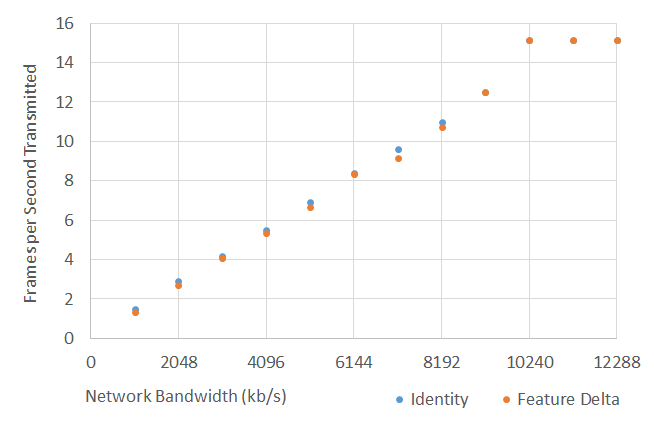
\includegraphics[width=\columnwidth]{figure3.png}
\caption{Framework tests with CPU at 2300MHz.}
\end{figure}

On the first run, the CPU clock speed was set to its maximum value. As Figure 1
demonstrates, the frame rate was proportional to the network speed at bandwidths
below 10Mbps, indicating that the network was the bottleneck.  At higher speeds,
the graph flattens as the camera reached its maximum possible frame rate.
There was no tangible difference in the frame rates between the operations,
showcasing the performance efficiency of the feature detection operation.

\begin{figure}
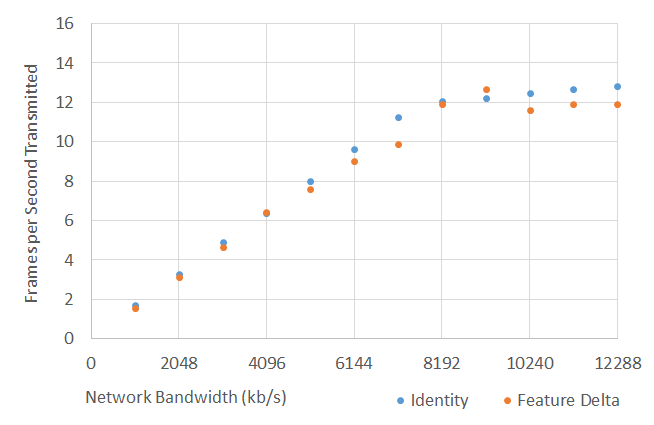
\includegraphics[width=\columnwidth]{figure4.png}
\caption{Framework tests with CPU at 800MHz.}
\end{figure}

With the clock speed throttled to 800MHz, the results were little different.  Up to about
9Mbps, the transmitted frame rate was quite close to that measured at 2300MHz.  At
higher bandwidths, the frame rate again flattened, this time about 2 frames per second
lower than in the first test.  As before, there was only a slight decrease in performance
between the two transformations.  Even in this test, the CPU usage remained well
below 100\%.

Although we have no direct basis for comparison between the Core i5 processor in the
test camera and the Raspberry Pi's ARM CPU, we can safely conclude that this framework
supports vision algorithms that run efficiently on computationally limited hardware, providing
acceptable frame rates even at relatively low network bandwidths.  The framework's transmission rate
is mainly network and camera-sensitive, giving us confidence that
this framework  will easily translate to high-end cell phone processors.

\begin{figure}
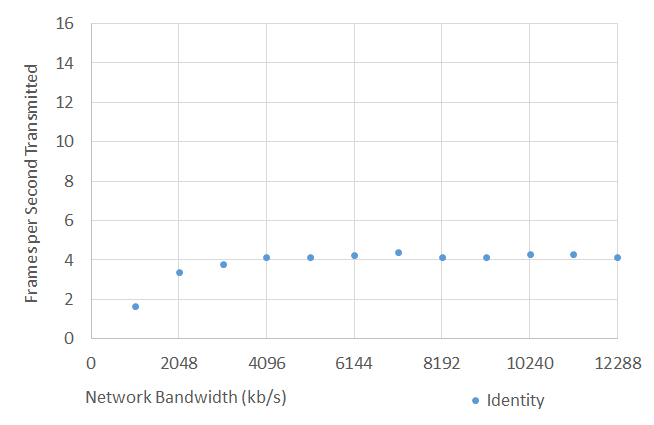
\includegraphics[width=\columnwidth]{figure5.png}
\caption{Identity transformation with CPU at 800MHz and spinning on locks rather than condition variables.}
\end{figure}

Interestingly, the original implementation of the push architecture required each pipeline stage to
spin on locks while waiting for information to enter its queue.  A subsequent iteration, the
one used to produce the data above, replaced this spinning with condition variables, resulting
in a 3x to 5x improvement in frame rates and significantly lower CPU utilization across all tests.
Figure 3 displays the frame rates from the Identity transformation using spinning on locks with
the processor speed set at 800MHz.  As
the graph clearly demonstrates, the simple change in synchronization primitive had a dramatic impact on
the overall performance of the framework.
